\documentclass[12pt, letterpaper]{article}

\usepackage[english]{babel} % sets the language and regional settings for english documents
\usepackage[utf8]{inputenc} % allows the use of utf-8 characters in the document
\usepackage[T1]{fontenc} % specifies the font encoding
\usepackage[margin=2cm]{geometry} % sets the page margins
\usepackage{makeidx} % enables the creation of indexes
\usepackage{natbib} % provides flexible bibliography support
\usepackage{url} % allows the use of urls
\usepackage{enumitem} % customizes the appearance of lists
\usepackage{listings} % provides syntax highlighting for code listings
\usepackage[dvipsnames]{xcolor} % allows the use of colors
\usepackage{parskip} % modifies paragraph spacing
\usepackage{graphicx} % enables the inclusion of graphics
\usepackage{tikz} % allows the creation of graphics and diagrams
\usepackage{float}
\usepackage{hyperref} % enables the creation of hyperlinks
\usepackage{amsmath} % provides additional math environments and commands
\usepackage{circuitikz} % allows the creation of electrical circuits
\usepackage{adjustbox} % adjusts the size of the circuit diagrams
\usepackage{arydshln} % allows the use of dashed lines in tables

\usetikzlibrary{shapes.geometric, positioning}

\lstset{
	language=sql,
	basicstyle=\ttfamily\small,
	keywordstyle=\color{blue},
	commentstyle=\color[rgb]{0,0.5,0},
	stringstyle=\color{red},
	numbers=left,
	numberstyle=\tiny\color{gray},
	stepnumber=1,
	numbersep=10pt,
	backgroundcolor=\color{white},
	showspaces=false,
	showstringspaces=false,
	breaklines=true,
	frame=single,
	tabsize=2, captionpos=b, lineskip=-1pt,
	extendedchars=true,
	literate={á}{{\'a}}1 {é}{{\'e}}1 {í}{{\'i}}1 {ó}{{\'o}}1 {ú}{{\'u}}1 {á}{{\'a}}1 {é}{{\'e}}1 {í}{{\'i}}1 {ó}{{\'o}}1 {ú}{{\'u}}1 {ñ}{{\~n}}1 {ñ}{{\~n}}1 {¿}{{\textquestiondown}}1 {¡}{{\textexclamdown}}1
}

\graphicspath{ {./img/} } % sets the path for the graphics

\newlist{biblio}{enumerate}{1}
\setlist[biblio,1]{label=[\arabic*]}

\makeindex

\begin{document}

\begin{titlepage}

	\begin{tikzpicture}[remember picture,overlay]
		\node[anchor=north west, inner sep=30] at (current page.north west) {
			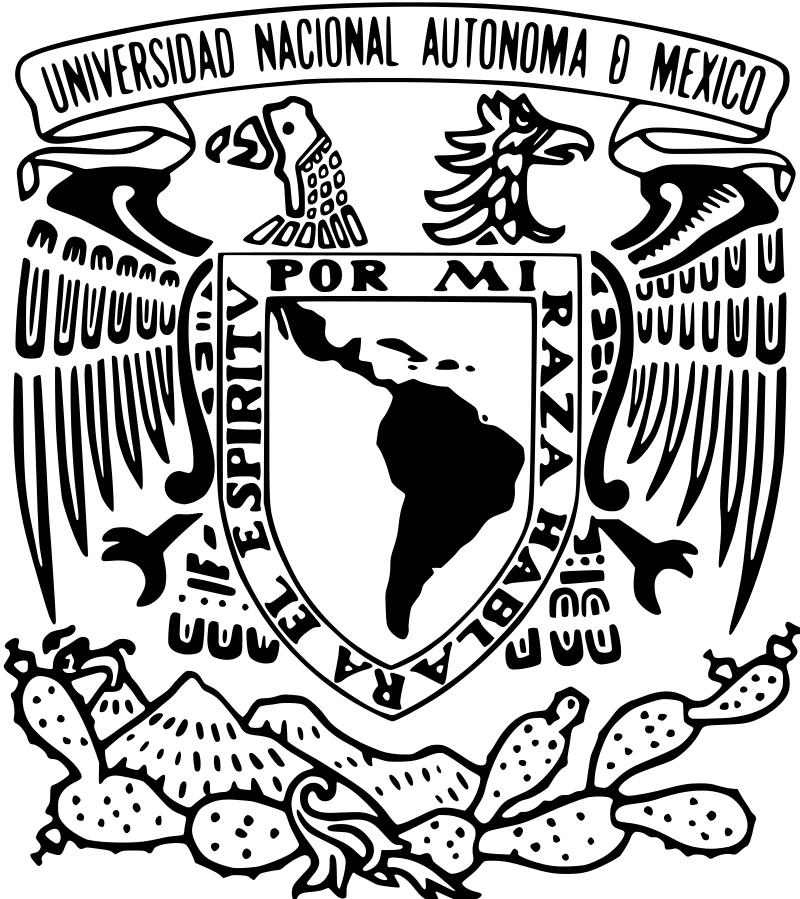
\includegraphics[width=4cm]{escudoUNAM.png}
		};

		\node[anchor=north east, inner sep=30] at (current page.north east) {
			
\includegraphics[width=4cm]{escudoFI.png}
		};
	\end{tikzpicture}

	\begin{center}
		\vspace*{3cm}

		\Huge
		\textbf{Compiler - Final Project}

		\vspace{2.5cm}

		\Huge
		\textbf{Facultad de Ingeniería}\\
		Compilers\\
		Semester 2025-2\\

		\vspace{2.5cm}

		\textbf{Group:} 5

		\vspace{2.5cm}

		\Huge
		\textbf{Team 1 Teammates:}\\
		Calderón Olalde Enrique Job\\
		Salazar Islas Luis Daniel\\
		Tepal Briseño Hansel Yael\\
		Ugartechea González Luis Antonio\\
		\textbf{Due Date:} 08/06/2025
		\vspace{2.5cm}
	\end{center}

\end{titlepage}

\section{Introduction}

\subsection*{Problem Statement}

We where asked to create a compiler for a programming language, this compiler needed to be able to read a source code file, filter it through the different stages of compilation. The compiler should be able to do at least if statements and arithmetic operations.

\subsection*{Motivation}

We were motivated to work with a C based programming language, this because it is easier to read and write. Nevertheless, we need to keep in mind that these languages need to be translated to machine code, this is also a benefit from the C base. Thanks to the structure, we are able to make the bridge between human-readable code and the machine-executable instructions.

\subsection*{Objectives}

Some of the objectives of the general assignment are:

\begin{itemize}
	\item create a string of tokens that can be used to represent the source code.
	\item produce a parse tree that represents the structure of the source code.
	\item produce an abstract syntax tree that represents the structure of the source code.
	\item produce an intermediate representation of the source code.
	\item produce an executable file.
	\item the executable file should be able to run the code written in the source code file.
\end{itemize}

\section{Theoretical Framework}

\subsection*{Compiler Architecture and Design}

A compiler is a complex software system that translates programs written in a high-level programming language into machine code or another lower-level representation. The compilation process is traditionally divided into several distinct phases, each with specific responsibilities and well-defined interfaces. Our implementation follows the classical multi-phase compiler architecture, consisting of five main components that work sequentially to transform source code into executable assembly code.

\subsubsection*{Multi-Phase Compilation Pipeline}

The compilation process in our implementation follows a linear pipeline architecture where each phase processes the output of the previous phase:

\begin{enumerate}
    \item \textbf{Lexical Analysis Phase}: transforms raw source code into a stream of tokens
    \item \textbf{Syntax Analysis Phase}: converts tokens into an abstract syntax tree (AST)
    \item \textbf{Semantic Analysis Phase}: validates semantic correctness and builds symbol tables
    \item \textbf{Intermediate Code Generation Phase}: transforms AST into intermediate representation (IR)
    \item \textbf{Code Generation Phase}: converts IR into target machine assembly code
\end{enumerate}

This modular approach provides several advantages including separation of concerns, easier debugging and testing, and the ability to make small changes to the compiler to adapt new features.

\subsection*{Lexical Analysis Theory}

\subsubsection*{Regular Languages}

Lexical analysis is based on the theory of regular languages. Each token type in our language is defined by a regular expression that describes the pattern of characters that form valid instances of that token type. The lexical analyzer uses these patterns to scan the input character stream and identify tokens.

Our implementation uses Python's \texttt{re} module, which implements a regular expression engine. The token specification includes:

\begin{itemize}
    \item \textbf{Keywords}: fixed strings like \texttt{if}, \texttt{else}, \texttt{while}, \texttt{int}, \texttt{return}, \texttt{print}
    \item \textbf{Identifiers}: pattern \texttt{[a-za-z\_][a-za-z0-9\_]*} for variable and function names
    \item \textbf{Constants}: pattern \texttt{-?[0-9]+} for integer literals
    \item \textbf{Operators}: multi-character operators such as \texttt{==}, \texttt{!=}, \texttt{<=}, \texttt{>=}, \texttt{\&\&}, \texttt{||}
    \item \textbf{Literals}: string patterns enclosed in quotes with escape sequence support
    \item \textbf{Punctuation}: single-character delimiters and brackets
\end{itemize}

\subsubsection*{Tokenization Process}

The tokenization process uses a longest-match principle implemented through a combined regular expression. All token patterns are concatenated using the alternation operator (\texttt{|}) with named capture groups, allowing the lexer to identify both the token type and value in a single pass through the input.

\subsection*{Syntax Analysis Theory}

\subsubsection*{Context-Free Grammars}

Syntax analysis is based on our context-free grammar (CFG). Our language is defined by a context-free grammar that specifies the syntactic structure of valid programs. The grammar uses a notation to define production rules that describe how complex language constructs are formed from simpler components.

The grammar for our C-based language includes productions for:

\begin{itemize}
    \item program structure
    \item statement types
    \item control flow constructs
    \item function definitions and calls
\end{itemize}

\subsubsection*{Recursive Descent Parsing}

Our parser implementation uses the recursive descent parsing technique, which is a top-down parsing method that constructs the parse tree from the root down to the leaves. Each non-terminal in the grammar corresponds to a parsing method that recognizes that syntactic construct.

The recursive descent approach offers several advantages:

\begin{itemize}
    \item direct correspondence between grammar rules and parsing methods
    \item easy to implement and understand
    \item good error recovery capabilities
\end{itemize}

\subsubsection*{Abstract Syntax Trees}

The parser constructs an Abstract Syntax Tree (AST) as its primary output. The AST is a tree representation of the syntactic structure of the program where:

\begin{itemize}
    \item each node represents a language construct (statement, expression, declaration)
    \item leaf nodes represent terminals (identifiers, constants, operators)
    \item internal nodes represent syntactic categories and their relationships
    \item irrelevant syntactic details (like parentheses and keywords) are abstracted away
\end{itemize}

\subsection*{Semantic Analysis Theory}

\subsubsection*{Symbol Tables and Scope Management}

Semantic analysis uses symbol table data structures to track identifier declarations and their properties throughout the compilation process. Our implementation uses a stack-based symbol table that supports nested scopes:

\begin{itemize}
    \item \textbf{Function Scope}: contains local variable declarations within functions
    \item \textbf{Block Scope}: supports nested scopes within control structures
\end{itemize}

Each symbol table entry contains:

\begin{itemize}
    \item identifier name
    \item type
    \item scope level
\end{itemize}

\subsubsection*{Type Checking and Semantic Validation}

The semantic analyzer performs several types of validation:

\begin{enumerate}
    \item \textbf{Declaration Checking}: ensures all identifiers are declared before use
    \item \textbf{Type Checking}: validates type compatibility in expressions and assignments
    \item \textbf{Scope Resolution}: ensures identifiers are used within their valid scope
\end{enumerate}

\subsubsection*{Visitor Pattern Implementation}

The semantic analyzer uses the Visitor design pattern to traverse the AST.\@

\subsection*{Intermediate Code Generation Theory}

\subsubsection*{Three-Address Code}

Our intermediate representation is based on three-address code (TAC), a form of intermediate code where each instruction has at most three operands. This representation has several advantages:

\begin{itemize}
    \item explicit representation of intermediate values using temporary variables
    \item easy translation to assembly language
    \item suitable for optimization passes
    \item machine-independent representation
\end{itemize}

\subsubsection*{IR Instruction Set}

The intermediate representation includes the following instruction types:

\begin{itemize}
    \item \textbf{Assignment Instructions}: \texttt{x = y}, \texttt{x = 5}
    \item \textbf{Binary Operation Instructions}: \texttt{t1 = x + y}, \texttt{t2 = a == b}
    \item \textbf{Label Instructions}: \texttt{l2:}, \texttt{main:}
    \item \textbf{Jump Instructions}: \texttt{goto l2}, \texttt{if\_false t1 goto l3}
    \item \textbf{Function Instructions}: \texttt{call func}, \texttt{return x}
    \item \textbf{I/O Instructions}: \texttt{print x}, \texttt{print "hello"}
\end{itemize}

\subsubsection*{Control Flow Translation}

The IR generator translates high-level control structures into low-level jump instructions:

\begin{itemize}
    \item \textbf{Conditional Statements}: translated using conditional jumps with labels for if-else branches
    \item \textbf{Loop Constructs}: implemented using label-jump combinations for loop entry, condition checking, and exit
    \item \textbf{Function Calls}: represented as call instructions with proper label management
\end{itemize}

\subsection*{Code Generation Theory}

\subsubsection*{Target Architecture: x86-32}

Our code generator targets the x86-32 architecture running on Linux. Key architectural features utilized include:

\begin{itemize}
    \item \textbf{Register Set}: eax, ebx, ecx, edx for general computation; esp, ebp for stack management
    \item \textbf{Memory Model}: 32-bit linear addressing
    \item \textbf{Calling Convention}: standard x86 calling convention with stack-based parameter passing
\end{itemize}

\subsubsection*{Stack Frame Management}

The code generator implements standard stack frame management using the EBP (base pointer) register:

\begin{itemize}
    \item \textbf{Function Prologue}: save old ebp, set new ebp, allocate local variable space
    \item \textbf{Variable Access}: use ebp-relative addressing for local variables
    \item \textbf{Function Epilogue}: deallocate locals, restore ebp, return to caller
\end{itemize}

\subsubsection*{System Call Interface}

The generated code uses Linux system calls for I/O operations:

\begin{itemize}
    \item \textbf{sys\_write (4)}: for output operations (print statements)
    \item \textbf{sys\_exit (1)}: for program termination
    \item \textbf{interrupt 0x80}: software interrupt mechanism for system call invocation
\end{itemize}

\subsubsection*{Runtime Support Routines}

The code generator includes runtime support routines for operations not directly supported by the instruction set:

\begin{itemize}
    \item \textbf{Integer to String Conversion}: implements division-based algorithm for printing integers
    \item \textbf{String Output}: handles utf-8 encoded string literals with escape sequence processing
    \item \textbf{Memory Management}: manages static data section for string literals and buffers
\end{itemize}

\subsection*{Language Design Constraints}

Our simplified C-based language has specific design constraints that influenced the theoretical approach:

\begin{itemize}
    \item \textbf{Single Data Type}: only 32-bit signed integers are supported, simplifying type checking and code generation
    \item \textbf{No Function Parameters}: functions cannot accept parameters, eliminating parameter passing complexity
    \item \textbf{No Dynamic Memory}: no pointers or arrays, resulting in purely stack-based memory management
    \item \textbf{Limited Control Flow}: no for loops or goto statements, using only if-else and while constructs
\end{itemize}

These constraints allow for a cleaner implementation while still demonstrating all major compiler construction principles.

\subsection*{Error Handling and Recovery}

\subsubsection*{Error Detection Strategies}

Each compilation phase implements specific error detection mechanisms:

\begin{itemize}
    \item \textbf{Lexical Errors}: invalid character sequences detected during tokenization
    \item \textbf{Syntax Errors}: grammar rule violations detected during parsing
    \item \textbf{Semantic Errors}: type mismatches and scope violations detected during semantic analysis
    \item \textbf{Code Generation Errors}: invalid IR instructions detected during assembly generation
\end{itemize}

\subsubsection*{Error Reporting}

The compiler provides detailed error messages including:

\begin{itemize}
    \item error type and description
    \item source location information
    \item context information to help identify the problem
\end{itemize}

\section{Development}

The compiler is developed in Python, we chose this language for its object-oriented capabilities to implement the different phases of compilation in a modular and understandable manner. Each phase is encapsulated in its own Python module facilitating independent development and testing.

\subsection*{Lexical Analyzer Implementation}

The lexical analyzer (lexer) is implemented using Python's built-in \texttt{re} module for regular expression matching.\@
The core of the lexer defines a list of token specifications, where each specification is a tuple containing a token type (e.g., \texttt{KEYWORD}, \texttt{IDENTIFIER}, \texttt{OPERATOR}) and a regular expression pattern that defines the lexeme for that token.\@
These individual regular expressions are combined into a single master regex using the OR operator (\texttt{|}), with named capture groups corresponding to each token type. This allows the \texttt{re.finditer()} method to efficiently scan the input source code and yield match objects.\@
For each match, the lexer determines the token type from the matched group name and extracts the token value. Comments and whitespace are identified and discarded. String literals are processed to remove their surrounding quotes. This approach directly implements the theoretical concept of using finite automata (as realized by the regex engine) to recognize regular language patterns in the input stream.

\subsection*{Parser Implementation}

The syntax analyzer (parser) is implemented as a recursive descent parser. This top-down parsing strategy is realized by a set of mutually recursive Python methods, where each method typically corresponds to a non-terminal symbol in the language\'s context-free grammar.\@
Abstract Syntax Tree (AST) nodes are defined as Python classes (e.g., \texttt{ProgramNode}, \texttt{FunctionNode}, \texttt{BinaryOpNode}), each encapsulating the relevant information for a specific language construct.\@
The parser consumes the stream of tokens produced by the lexer. As parsing methods are called, they check the current token against expected token types or values based on the grammar rules. If a rule is matched, the method consumes the corresponding tokens and recursively calls other parsing methods to process sub-constructs, building up AST nodes in the process. For instance, a method for parsing a binary expression would expect an operand, then an operator, then another operand, recursively calling an expression parsing method for the operands.\@
Error handling is incorporated by raising custom exceptions when the token stream does not conform to the expected syntax, providing messages about the nature and location of the error.

\subsection*{Semantic Analyzer Implementation}

The semantic analyzer is implemented to traverse the AST produced by the parser, performing validation checks and building symbol tables.\@
The Symbol Table is implemented as a Python class, typically using a list of dictionaries to represent the stack of scopes. Each dictionary maps identifier names to \texttt{Symbol} objects, which store information like the identifier\'s type and scope level. Methods are provided to \texttt{enter\_scope}, \texttt{exit\_scope}, \texttt{declare} a new symbol, and \texttt{lookup} an existing symbol.\@
The AST traversal is achieved using the Visitor design pattern. A \texttt{SemanticAnalyzer} class contains \texttt{visit\_NodeType} methods for each type of AST node. When the \texttt{analyze} method is called with the root of the AST, it dispatches to the appropriate visit method based on the node\'s type.\@
During traversal, these visit methods implement semantic rules:
\begin{itemize}
    \item For \texttt{DeclarationNode}, an identifier is added to the current scope in the symbol table.
    \item For \texttt{IdentifierNode}, a lookup is performed to ensure the identifier has been declared.
    \item For \texttt{AssignmentNode} and \texttt{BinaryOpNode}, type checking is performed to ensure compatibility between operands (though in our simplified language, this is mainly about ensuring variables are used in contexts appropriate for integers because the language just contains int)
    \item Function declarations and calls are checked for consistency.
\end{itemize}
Semantic errors, such as using an undeclared variable or re-declaring a variable in the same scope, result in custom \texttt{SemanticError} exceptions being raised.

\subsection*{Intermediate Code Generator Implementation}

The Intermediate Representation (IR) generator also employs the Visitor pattern to traverse the AST.\@
IR instructions (like \texttt{LabelInstr}, \texttt{AssignInstr}, \texttt{BinaryOpInstr}, \texttt{JumpInstr}) are defined as Python classes. Each class stores the components of a three-address-like instruction (e.g., target, source1, operator, source2).\@
The \texttt{IRGenerator} class maintains a list to which new IR instruction objects are appended. It also manages the creation of unique temporary variable names and labels needed for control flow.\@
As the visitor methods traverse the AST:
\begin{itemize}
    \item Expressions (e.g., \texttt{BinaryOpNode}) are translated into a sequence of IR instructions that compute the expression\'s value, storing the result in a new temporary variable. The name of this temporary variable is then returned to be used by parent AST nodes.
    \item Assignment statements generate \texttt{AssignInstr} objects.
    \item Control flow constructs like \texttt{ConditionalNode} (if statements) and \texttt{WhileNode} (while loops) generate \texttt{LabelInstr} for targets and \texttt{ConditionalJumpInstr} or \texttt{JumpInstr} to manage the flow of execution. New labels are generated as needed.
    \item Function definitions generate entry labels and return instructions.
\end{itemize}
The result of this phase is a flat list of Python objects, each representing an IR instruction in sequential order.

\subsection*{Code Generator Implementation}

The final code generator takes the list of IR instruction objects and translates them into x86 assembly language for a Linux target.\@
The \texttt{CodeGenerator} class in Python maintains separate lists for the \texttt{.data} and \texttt{.text} sections of the assembly file.\@
It iterates through the IR instructions:
\begin{itemize}
    \item A key aspect is managing variable locations. For each function, it first collects all local variables and temporary variables used. Based on this, it calculates the required stack space for the function\'s stack frame. Variables are then mapped to offsets from the base pointer (\texttt{ebp}).
    \item \texttt{LabelInstr} from the IR translates directly to assembly labels.
    \item \texttt{AssignInstr} translates to \texttt{mov} instructions, moving data between registers, memory locations (stack variables), and immediate values.
    \item \texttt{BinaryOpInstr} translates to corresponding x86 arithmetic or comparison instructions (e.g., \texttt{add}, \texttt{sub}, \texttt{imul}, \texttt{idiv}, \texttt{cmp} followed by \texttt{sete}, \texttt{setne}, etc.). Operands are loaded into registers (typically \texttt{eax}, \texttt{ebx}), the operation is performed, and the result is stored back into the target variable\'s stack location.
    \item \texttt{JumpInstr} and \texttt{ConditionalJumpInstr} translate to \texttt{jmp}, \texttt{je}, \texttt{jne}, etc., using the labels defined in the IR.\@
    \item \texttt{PrintInstr} is handled by generating calls to helper assembly routines for printing integers or by directly using Linux \texttt{sys\_write} system calls for string literals. String literals are added to the \texttt{.data} section with unique labels.
    \item Function prologues (setting up \texttt{ebp}, allocating stack space) and epilogues (restoring \texttt{ebp}, deallocating stack space, \texttt{ret}) are generated for each function. The \texttt{main} function\'s return is translated into a program exit sequence using the \texttt{sys\_exit} system call.
\end{itemize}
Helper routines, such as \texttt{print\_integer} (which converts an integer in a register to its ASCII string representation and prints it using \texttt{sys\_write}) and \texttt{print\_newline}, are appended to the \texttt{.text} section. The final assembly code is produced by concatenating the \texttt{.data} and \texttt{.text} sections.

This modular Python implementation allows each theoretical concept of compilation to be clearly mapped to a corresponding part of the codebase, making the compiler\'s structure and operation transparent and maintainable.

\subsection*{Test}

To ensure the correctness and robustness of each component of the compiler (Lexer, Parser, Semantic Analyzer, Intermediate Code Generator, and Code Generator), a comprehensive suite of unit tests was developed using Python's built-in \texttt{unittest} framework. These tests cover a wide range of scenarios, including valid inputs, edge cases, and error conditions for each phase.

The tests are organized within the \texttt{tests/} directory, with separate files for each compiler module (e.g., \texttt{test\_lexer.py}, \texttt{test\_parser.py}).

\subsubsection*{Running the Tests}
All tests can be executed from the root directory of the project using the following command:

\begin{lstlisting}[language={}, basicstyle=\ttfamily\footnotesize, frame=none, breaklines=true]
python -m unittest discover -s tests
\end{lstlisting}

This command instructs the \texttt{unittest} module to:
\begin{itemize}
    \item \texttt{discover}: Automatically find test files.
    \item \texttt{-s tests}: Start discovery in the \texttt{tests} directory.
\end{itemize}

The output of the test suite, indicating the number of tests run and their status (e.g., OK, FAILED, ERROR), is typically printed to the standard output and standard error. To capture this output for review, it can be redirected to a file. For example, to save the results to \texttt{tests/test\_result.txt}:

\begin{lstlisting}[language={}, basicstyle=\ttfamily\footnotesize, frame=none, breaklines=true]
python -m unittest discover -s tests > tests/test_result.txt 2>&1
\end{lstlisting}

\subsubsection*{Expected Test Output}
A successful run of all tests will produce output similar to the following in \texttt{tests/test\_result.txt}:

\begin{lstlisting}[language={}, basicstyle=\ttfamily\footnotesize, frame=none, breaklines=true]
..............................................................................................
----------------------------------------------------------------------
Ran 94 tests in 0.015s

OK
\end{lstlisting}

This output indicates that all 94 tests passed successfully. The series of dots (\texttt{...................}) represents individual test cases passing.
\section{Results}

We achieved our expected goals, the compiler is able to receive a source code file and then output an executable file which we can run in our personal computers.
We design many test cases to test the compiler, these test cases are designed to cover all the features of the language, including arithmetic operations, if statements, while loops, and function calls. The compiler is able to handle all of these test cases without any issues.



\section{Conclusions}

In conclusion, this project was successfully completed, and we had a better approach of how modern compilers work, which complex processes a
\section{References}

% \begin{biblioment, we will set our own objectives to guide the development of the compiler.}
% 	%for: https://www.poli.edu.co/blog/poliverso/diseno-digital-que-es
% 	\item \textit{diseño digital: qué es y por qué es importante.} (2021, august 26). poliverso. retrieved october 16, 2024, from: \textcolor{blue}{\underline{\url{https://www.poli.edu.co/blog/poliverso/diseno-digital-que-es}}}
% 	%for: https://www.sky6cancun.com/marketing/diseno-grafico/diseno-digital-que-es-y-para-que-sirve/
% 	\item \textit{diseño digital: qué es y para qué sirve.} (2021, august 26). sky6cancún. retrieved october 16, 2024, from: \textcolor{blue}{\underline{\url{https://www.sky6cancun.com/marketing/diseno-grafico/}}}
% \end{biblio}

\end{document}
